\documentclass[UTF8,a4paper,12pt]{ctexart}

\usepackage[a4paper,margin=2.35cm,headheight=15pt]{geometry}
\usepackage{fontspec}
\setmainfont{TeX Gyre Termes}
\setsansfont{TeX Gyre Heros}
\setmonofont{DejaVu Sans Mono}
\setCJKmainfont{Noto Serif CJK SC}
\setCJKsansfont{Noto Sans CJK SC}
\setCJKmonofont{Noto Sans Mono CJK SC}

\usepackage{graphicx}
\usepackage{booktabs}
\usepackage{longtable}
\usepackage{tabularx}
\usepackage{array}
\usepackage{amsmath}
\usepackage{amssymb}
\usepackage{float}
\usepackage{caption}
\usepackage{subcaption}
\usepackage{enumitem}
\usepackage{fancyhdr}
\usepackage{hyperref}
\usepackage{bookmark}
\usepackage{tikz}
\usepackage{pgfplots}
\pgfplotsset{compat=1.18}
\usepackage{xcolor}

\hypersetup{
  colorlinks=true,
  linkcolor=black,
  citecolor=black,
  urlcolor=blue,
  pdftitle={赣江西支特大桥水文与行洪一维水动力分析报告},
  pdfauthor={项目计算稿}
}

\pagestyle{fancy}
\fancyhf{}
\lhead{赣江西支特大桥水文与行洪分析}
\rhead{HEC-RAS 1D 稳定流 / CAD01直接设计河床}
\cfoot{\thepage}

\renewcommand{\arraystretch}{1.25}
\setlength{\parindent}{2em}
\setlength{\parskip}{0.25em}
\captionsetup{font=small,labelfont=bf}

\newcommand{\mthreeps}{\mathrm{m^3/s}}
\newcommand{\WSE}{\mathrm{WSE}}
\newcommand{\modelversion}{v3-CAD01}

\title{\bfseries 赣江西支特大桥水文与行洪一维水动力分析报告\\[0.8em]
\large HEC-RAS 1D 稳定流五工况与 CAD 01 直接设计河床验证}
\author{项目计算稿}
\date{2026年8月30日}

\begin{document}

\maketitle
\thispagestyle{empty}
\vfill
\begin{center}
\begin{minipage}{0.88\textwidth}
\small
\textbf{报告定位：}本报告基于现有 CAD/DWG、五个实测断面及给定设计行洪参数，采用 HEC-RAS 7.0.1 一维稳定流比较现状河床、三种防冲刷工况与设计河床工况。当前设计河床不再采用人工受约束重建，而直接使用 01 号防冲刷 CAD 中标注为“中地面线（建设期）”的完整断面线。报告用于一维行洪影响筛选，不替代显式桥梁局部水力模型、二维流场或桥墩冲刷计算。
\end{minipage}
\end{center}
\vfill
\clearpage

\begin{abstract}
本项目采用 HEC-RAS 7.0.1 一维稳定流作为主求解器，以 Python 完成 CAD 证据恢复、几何构造、HDF 几何一致性审计、结果整理和独立量级校核。计算流量为 $Q=26{,}000\ \mthreeps$，基准 Manning 粗糙系数为 $n=0.030$，基准下游 Known WS 为 22.049342~m。

新的 CAD 审计确认：01 号《赣江西支特大桥抗冲刷防护（水下不分散混凝土）》图中，“中地面线（建设期）”文字通过引线直接指向一条完整河床折线；同图“上游地面线（现状）”与实测桥下断面形成 166 点对应关系，可建立 CAD 坐标到 station/elevation 的直接变换。由此恢复的设计河床同时严格命中 15\#/16\#/17\# 的 4.27/5.40/9.56~m 设计泥面表值。因此旧版“未找到完整设计河床、需用三个控制点和面积约束自行补线”的方法已经退役。

在 WSE=22.190~m 下，CAD 直接设计河床毛过水面积为 5934.568~m$^2$；扣除 280~m$^2$ 等效阻水后净面积为 5654.568~m$^2$。它与原表列 5980/5700~m$^2$ 均相差 45.432~m$^2$（约 0.76\%）。本报告采取完整 CAD 几何优先，不为强行满足表值而修改设计河床，并将该差异作为资料口径审计项。

HEC-RAS p05 HDF 的 RS=500 几何已与 CAD 直接设计河床逐点核对通过。基准边界下，设计河床工况在桥上游约 100~m 的 RS=600 得到 WSE=22.576809~m，相对现状增加 193.6~mm；桥下 RS=500 平均流速约 4.692~m/s。三种防护工况在 RS=600 的附加壅水仍分别约 2.525、3.803、6.382~mm。下游水位 $\pm0.50$~m 的历史计算仍可用于现状与三种防护，因为这四种几何没有变化；旧 DesignBed 边界结果来自已退役几何，本版不再引用，需用 CAD 直接设计河床重新计算后才能恢复该项敏感性结论。
\end{abstract}

\tableofcontents
\clearpage

\section{任务目标与成果边界}

\subsection{任务目标}
本次计算回答：在设计洪水流量 26000~m$^3$/s 下，现状河床、CAD 01 直接设计河床以及设置不同高度防冲刷设施后，桥位河段的一维水面线、平均流速、过流面积和上游壅水如何变化。

五个活动主工况见表~\ref{tab:cases}。

\begin{table}[H]
\centering
\caption{五个活动主工况}
\label{tab:cases}
\begin{tabular}{llr}
\toprule
工况 & 桥下河床来源 & 等效阻水面积 (m$^2$) \\
\midrule
现状河床 & 实测桥下断面 & 360 \\
0.5 m 防冲刷 & 实测桥下断面 & 380 \\
1.0 m 防冲刷 & 实测桥下断面 & 390 \\
2.0 m 防冲刷 & 实测桥下断面 & 410 \\
设计河床 & CAD 01“中地面线（建设期）”直接线 & 280 \\
\bottomrule
\end{tabular}
\end{table}

\subsection{成果边界}
当前成果属于\textbf{一维等效阻水行洪筛选模型}。它能够用于比较工况间整体水位和断面平均水力参数，但不能直接回答：
\begin{itemize}[leftmargin=2.2em]
  \item 桥墩周围局部最大流速、绕流和涡结构；
  \item 局部冲刷深度和冲刷坑发展；
  \item 桥面压力流、低弦控制或漫顶问题；
  \item 缺少正式下游水位--流量关系时的最终绝对设计洪水位。
\end{itemize}

\section{基础资料与 CAD 数据恢复}

\subsection{已有图纸与断面}
工作区包含 4 份原始 DWG，并已转换为程序可读 DXF。由五断面图恢复出 5 个关键横断面：上游 500~m、上游 100~m、桥下、下游 100~m、下游 500~m。HEC-RAS 河道桩号沿下游方向递减，关系见图~\ref{fig:reach-schematic}。

\begin{figure}[H]
\centering
\begin{tikzpicture}[x=0.012cm,y=1cm,>=stealth]
  \draw[->,thick] (0,0) -- (1000,0);
  \node[above] at (0,0.2) {上游};
  \node[above] at (1000,0.2) {下游};
  \foreach \x/\lab/\desc in {0/1000/上游500 m,400/600/上游100 m,500/500/桥下,600/400/下游100 m,1000/0/下游500 m}{
    \draw[thick] (\x,-0.35) -- (\x,0.35);
    \node[below,align=center] at (\x,-0.4) {RS=\lab\\\desc};
  }
  \draw[<->] (400,0.8) -- node[above]{约100 m} (500,0.8);
  \draw[<->] (500,0.8) -- node[above]{约100 m} (600,0.8);
\end{tikzpicture}
\caption{HEC-RAS 一维河段与五个关键断面示意}
\label{fig:reach-schematic}
\end{figure}

\subsection{CAD 图纸证据视图}
图~\ref{fig:cad-antiscour}--\ref{fig:cad-bridge-plan} 为脚本直接解析 DXF 实体后生成的工程图视图，用于固定“采用了哪些 CAD 信息”；原始 DWG/DXF 仍是最终图纸依据。

\begin{figure}[H]
\centering
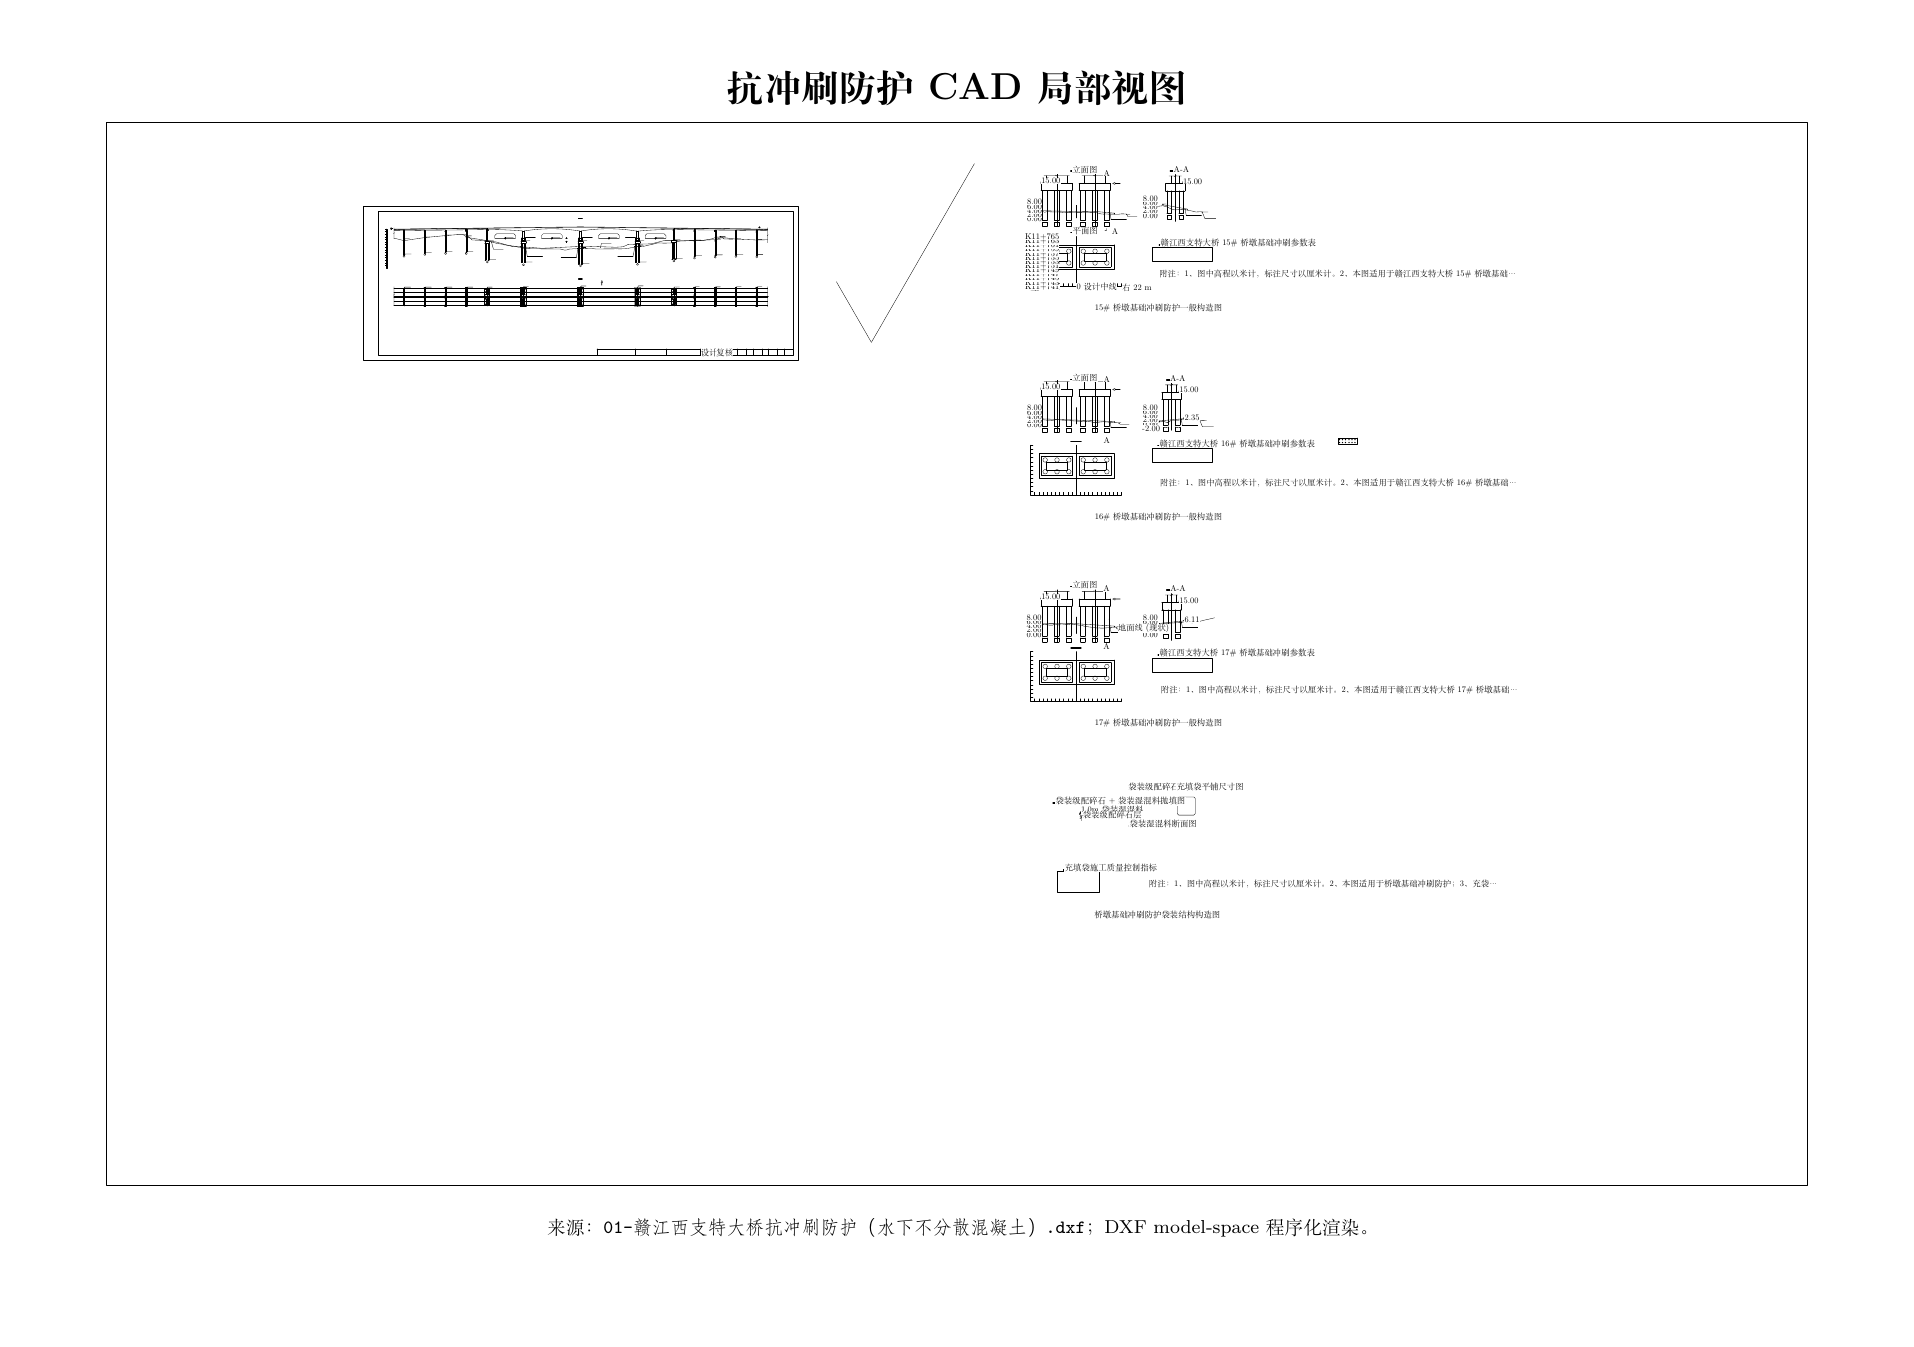
\includegraphics[width=0.96\textwidth]{figures/cad_antiscour.png}
\caption{01 号抗冲刷防护图 CAD/DXF 局部视图}
\label{fig:cad-antiscour}
\end{figure}

\begin{figure}[H]
\centering
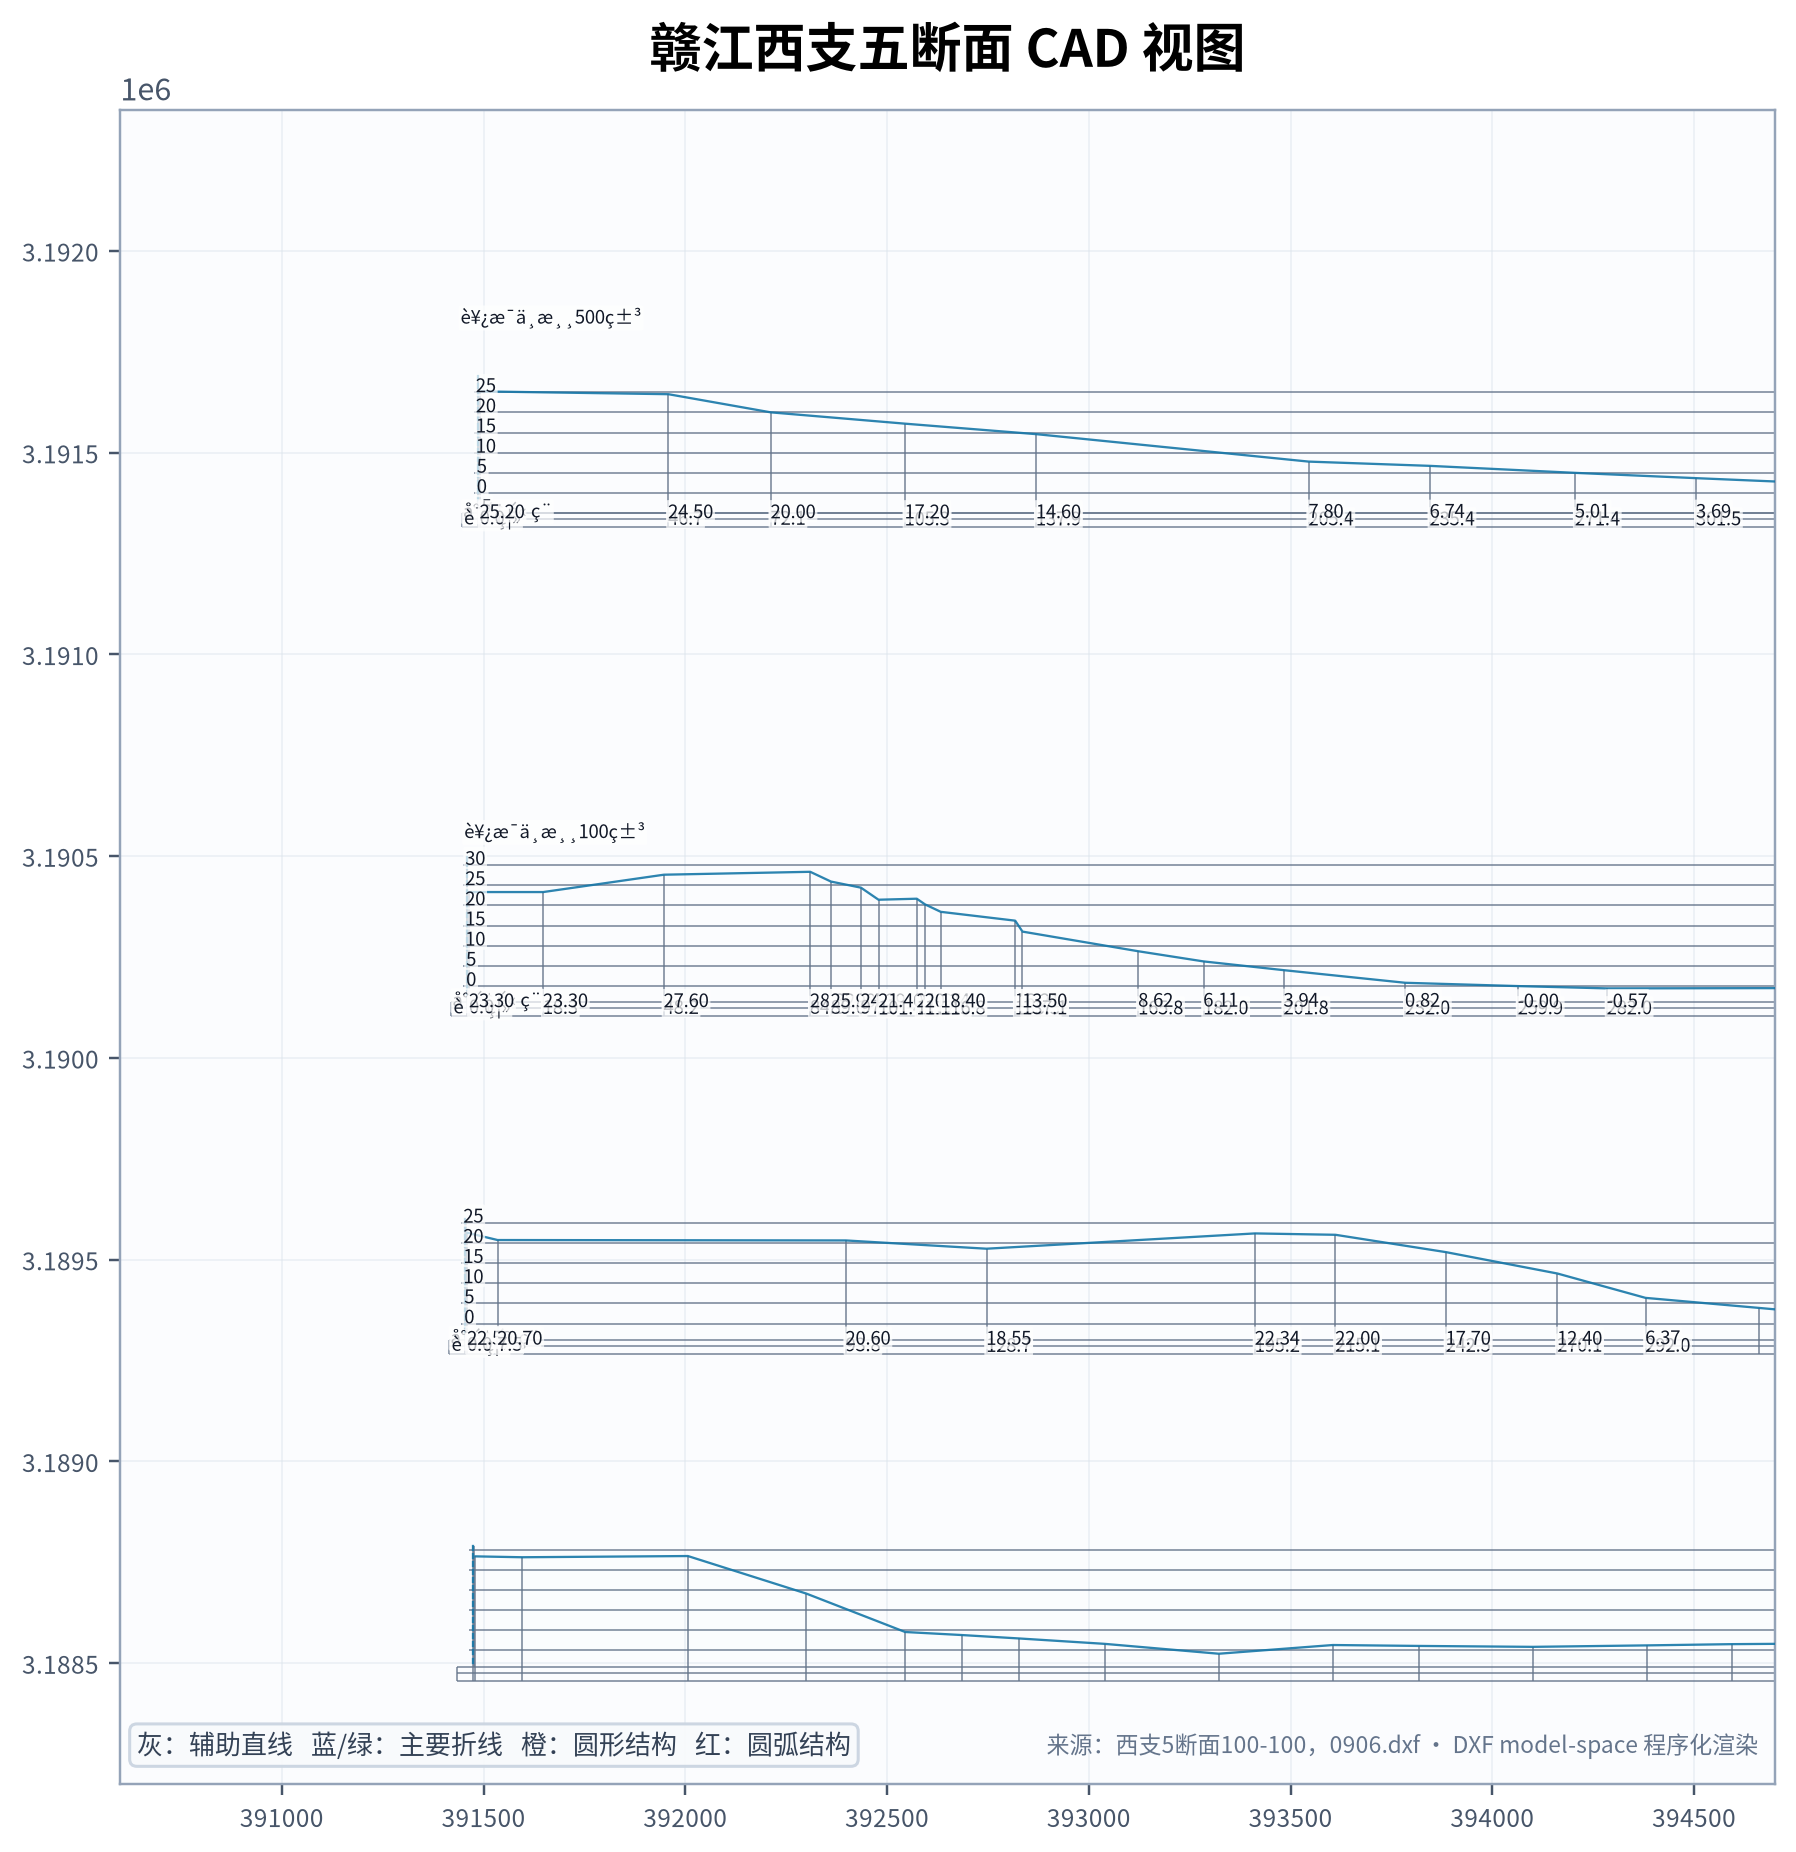
\includegraphics[width=0.96\textwidth]{figures/cad_five_sections.png}
\caption{赣江西支五个实测断面 CAD/DXF 视图}
\label{fig:cad-five-sections}
\end{figure}

\begin{figure}[H]
\centering
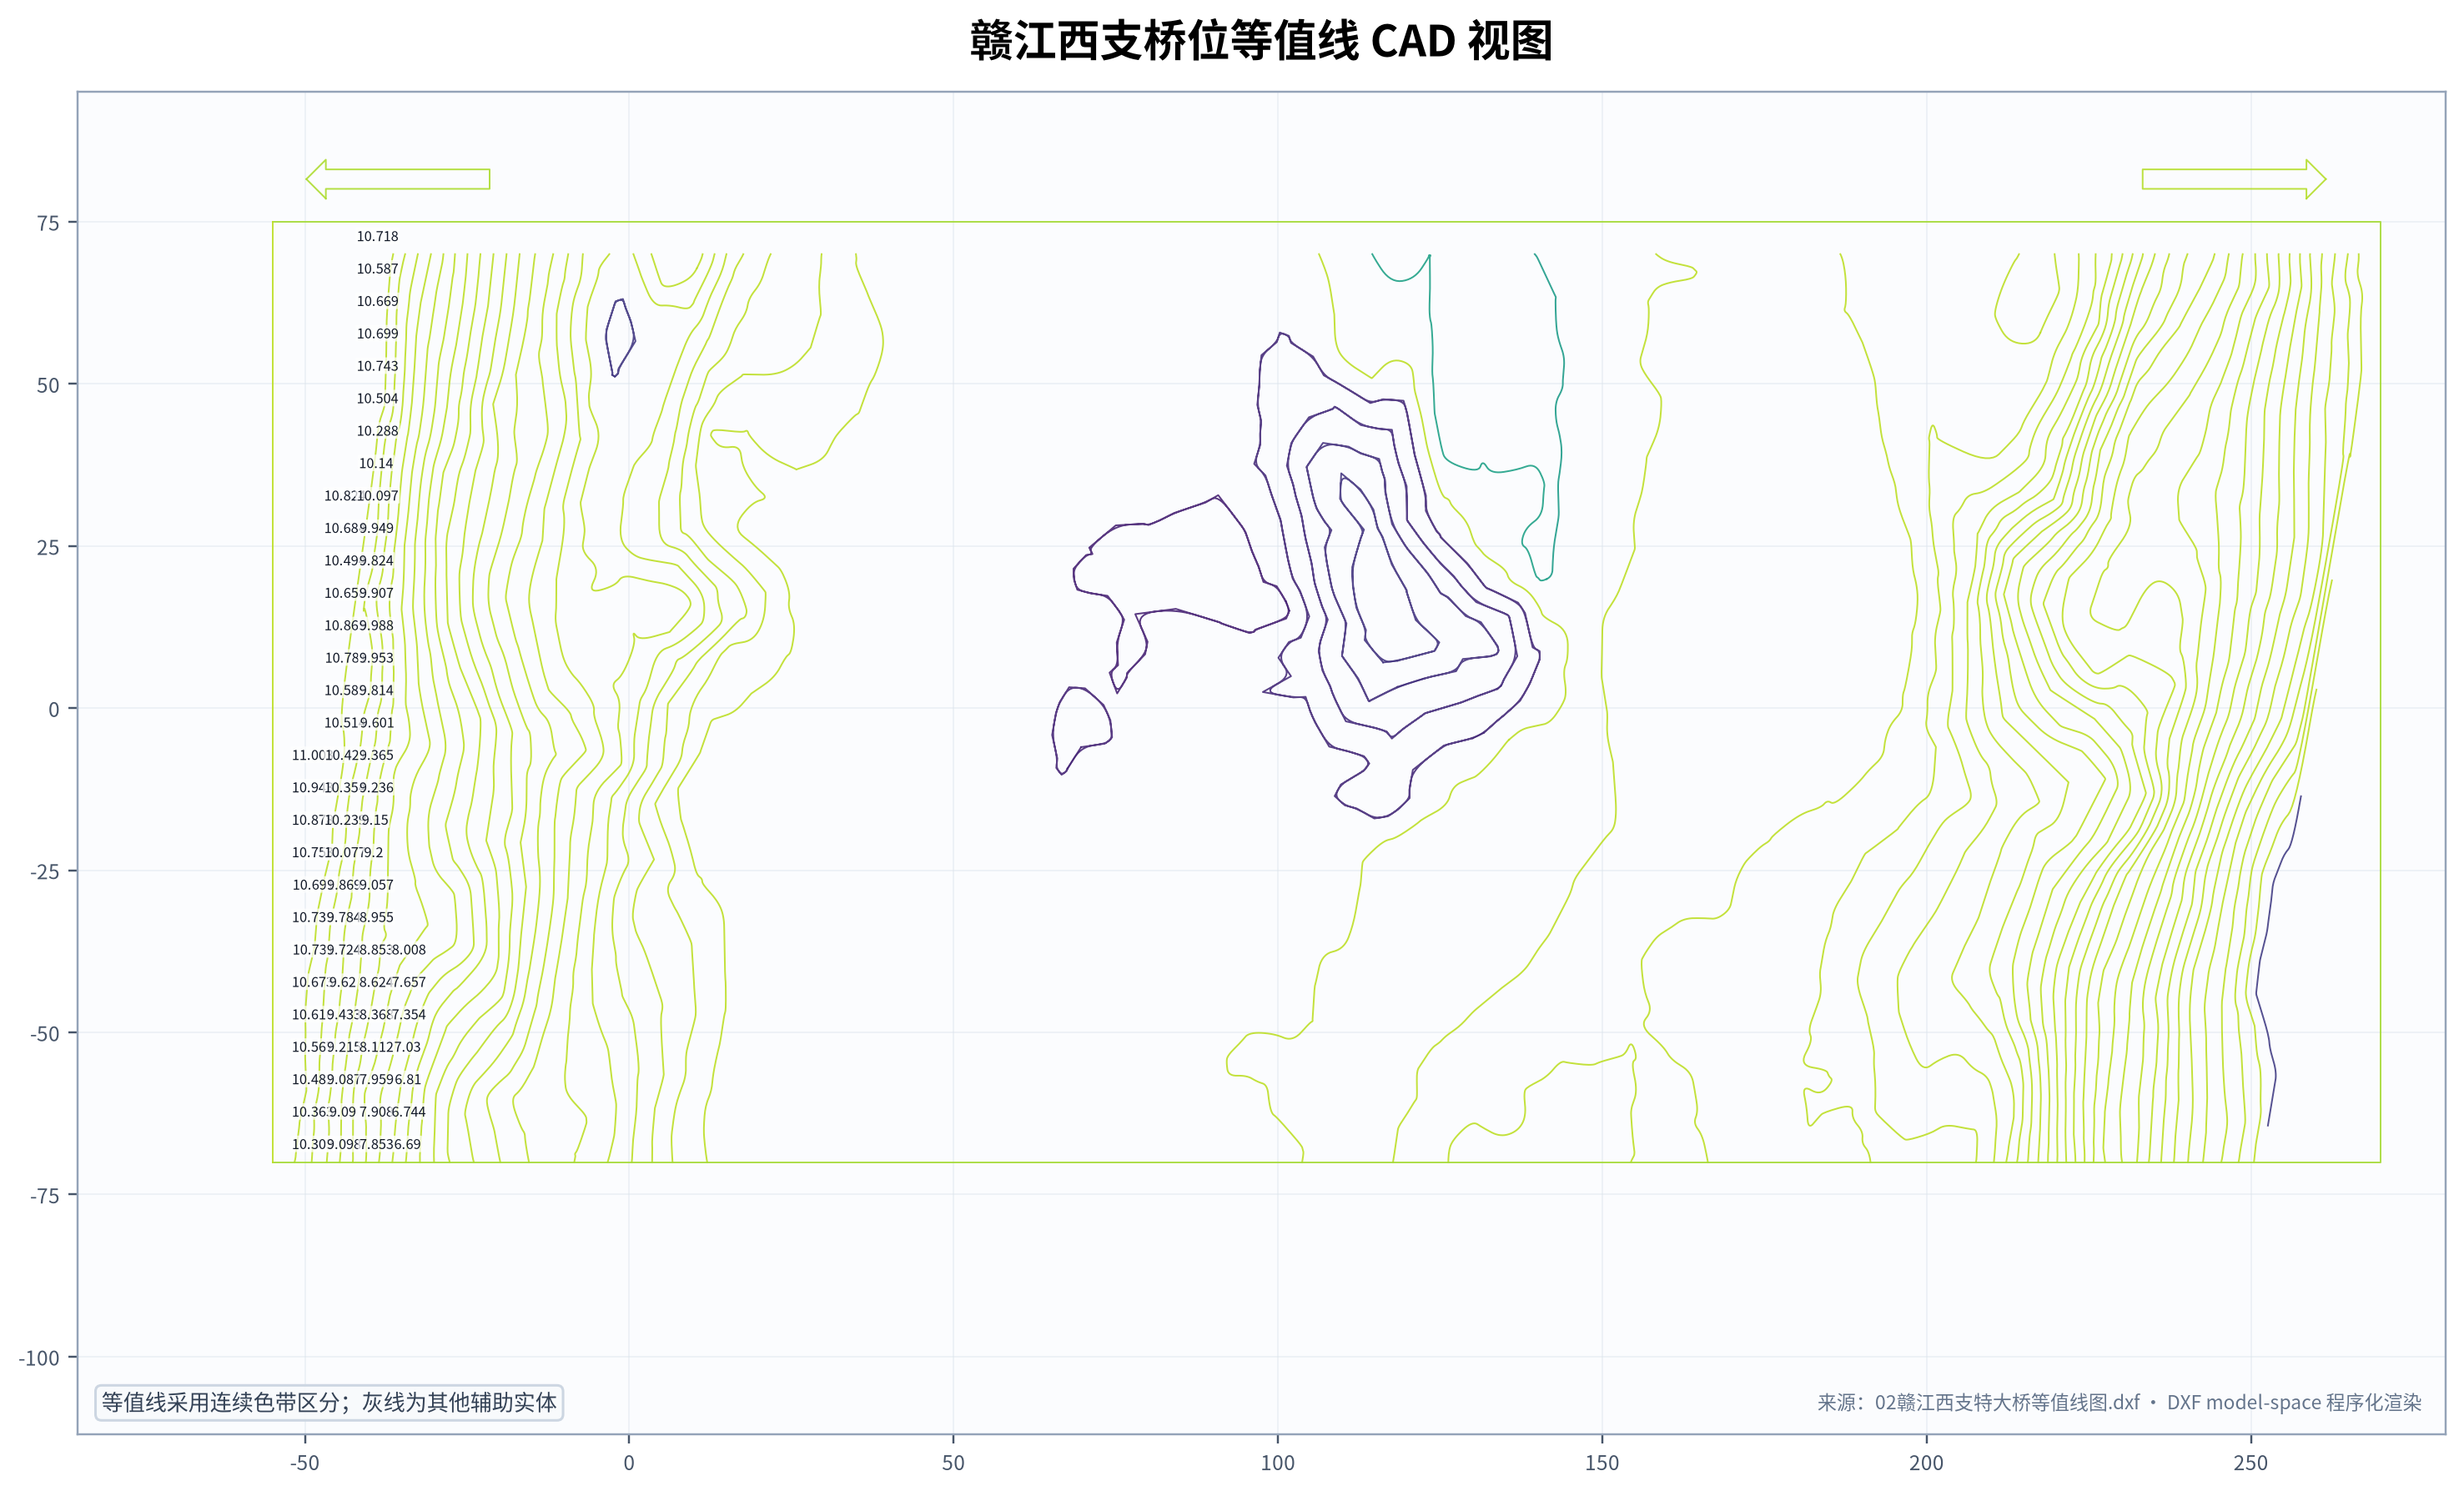
\includegraphics[width=0.96\textwidth]{figures/cad_contours.png}
\caption{赣江西支桥位等值线 CAD/DXF 视图}
\label{fig:cad-contours}
\end{figure}

\begin{figure}[H]
\centering
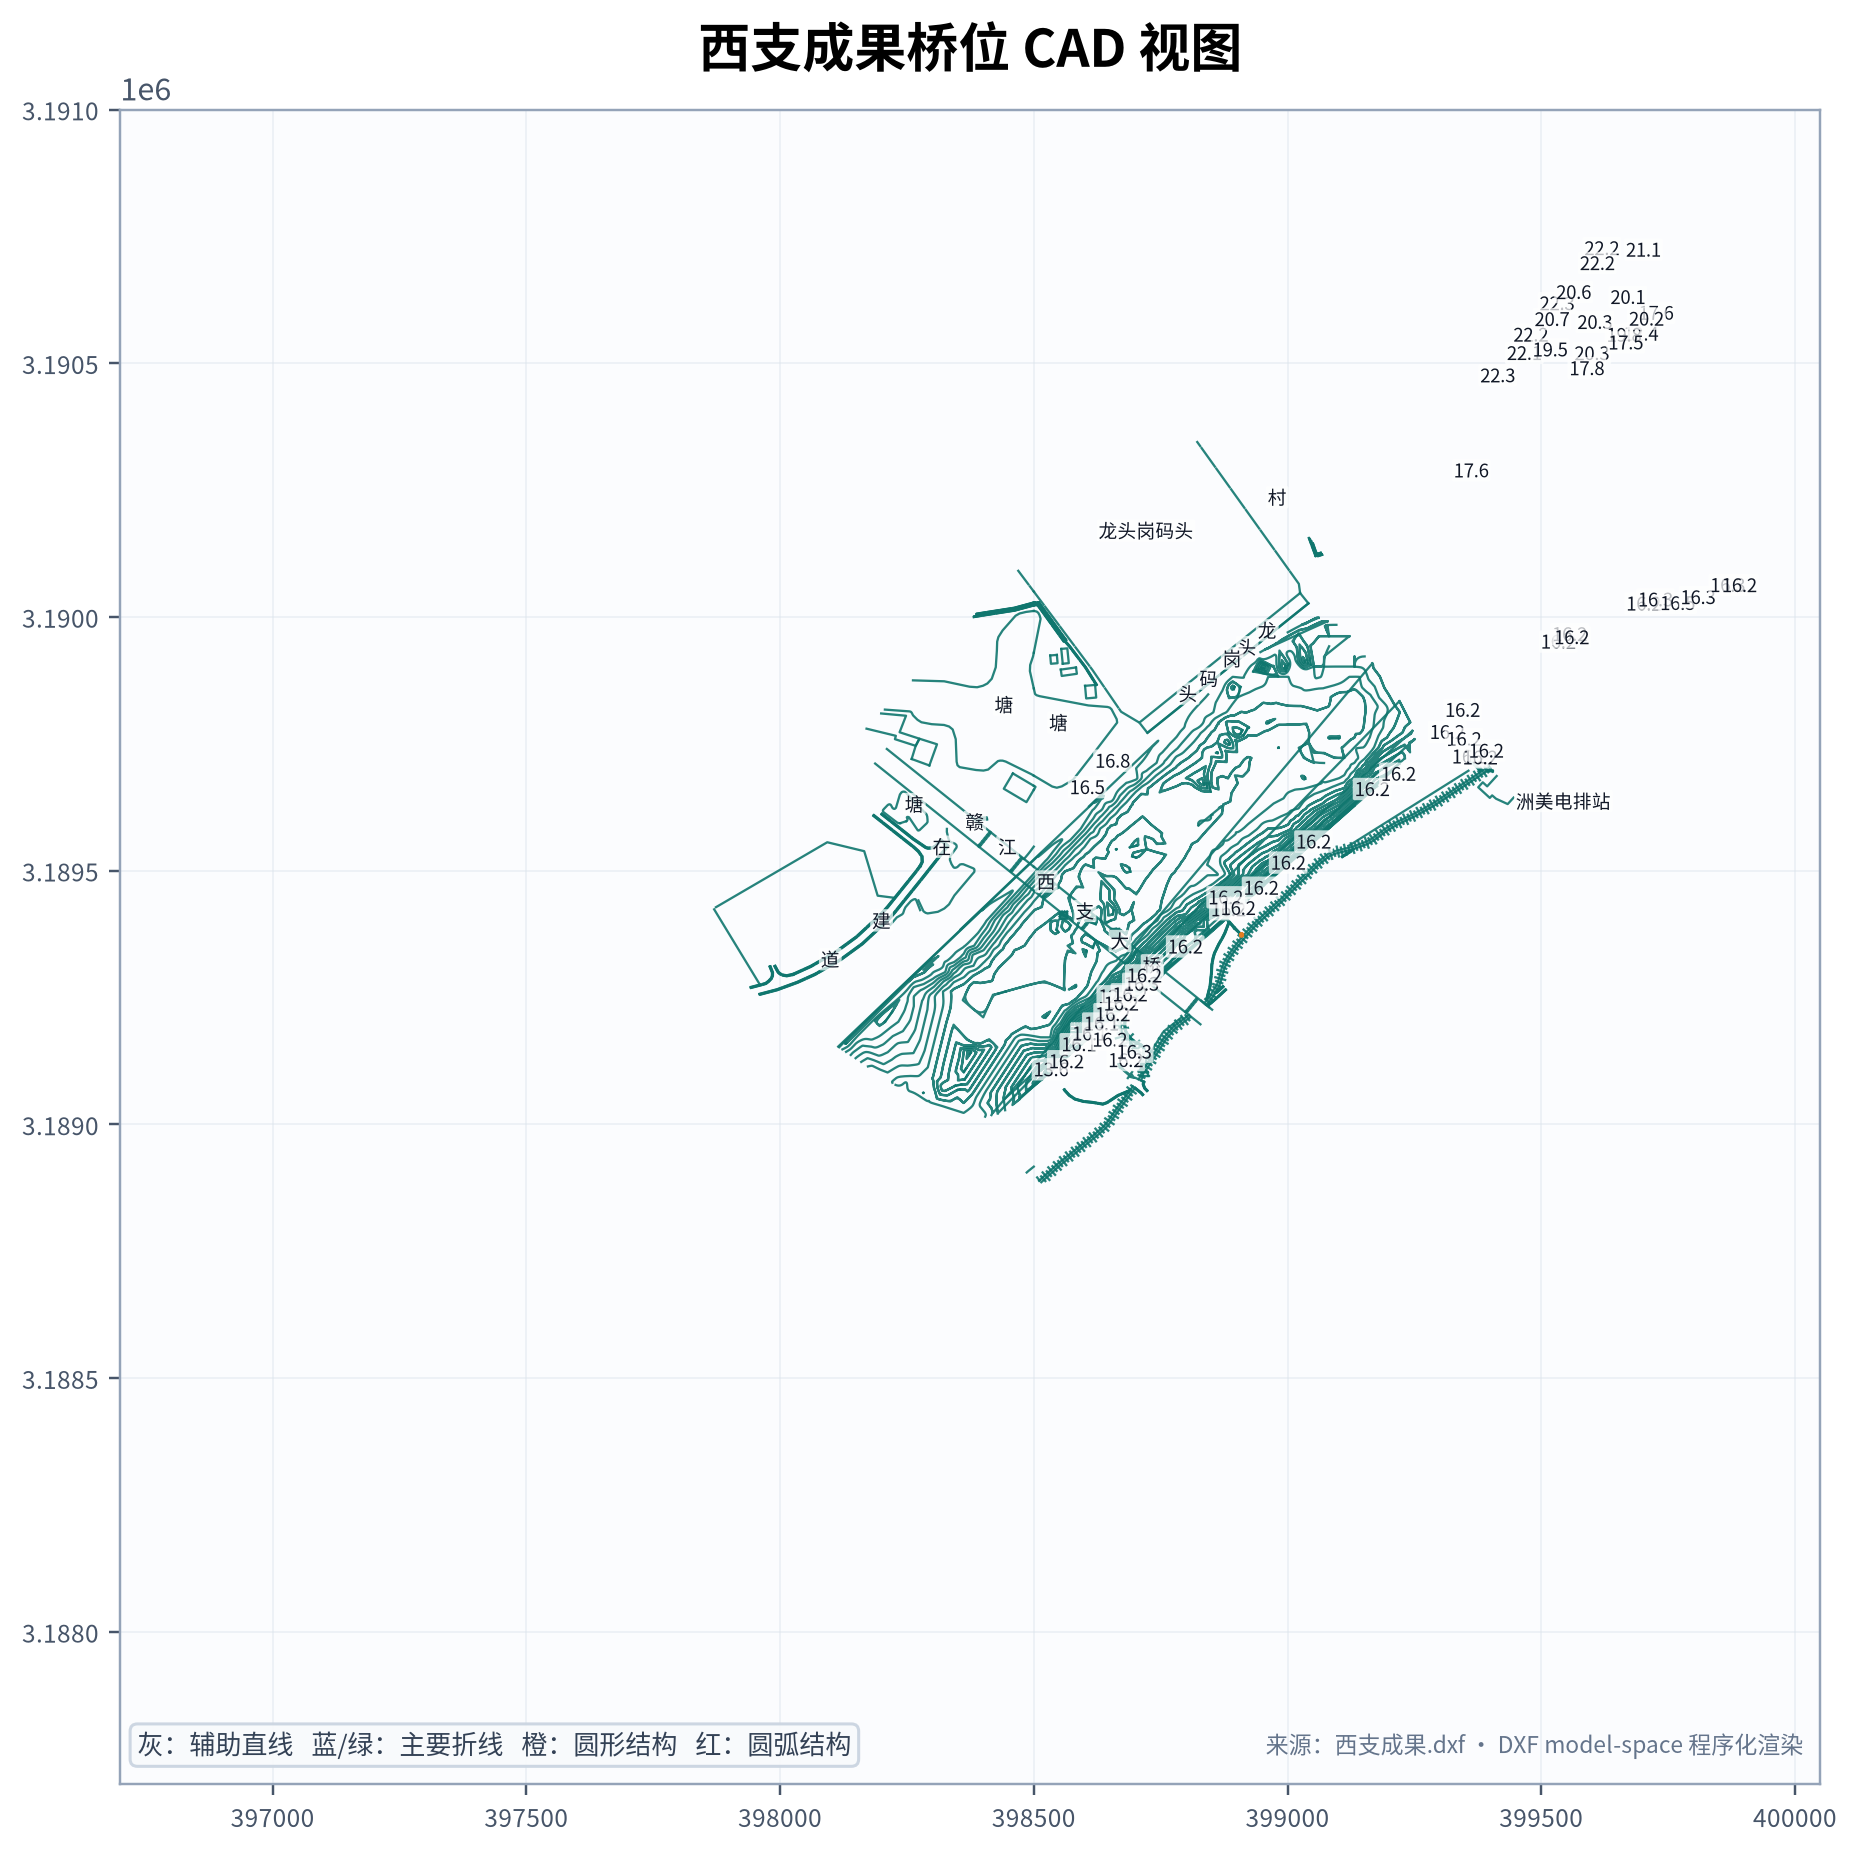
\includegraphics[width=0.96\textwidth]{figures/cad_bridge_plan.png}
\caption{西支成果图中的桥位 CAD/DXF 视图}
\label{fig:cad-bridge-plan}
\end{figure}

\section{CAD 01 直接设计河床证据链}

\subsection{语义标签、引线与完整河床线}
新的恢复过程以图纸语义而不是固定句柄作为首要定位依据。程序在 CAD 01 中找到文字“中地面线（建设期）”，沿其引线定位到被实际指向的完整 LWPOLYLINE；同时找到“上游地面线（现状）”作为坐标转换参考。

现状参考线有 166 个顶点，与处理后的桥下实测断面逐点对应。由对应点求得 station/elevation 变换后，将建设期完整河床直接变换到 HEC-RAS 断面坐标。活动设计河床 CSV 共保留 28 个有效断面点；恢复不使用“中心/局部/分布型”等人工补线方案。

\subsection{设计泥面表值交叉核验}
CAD 基础冲刷参数表中的 15\#/16\#/17\# 设计泥面高程作为独立核验量。直接设计河床对应值见表~\ref{tab:pier-control}。

\begin{table}[H]
\centering
\caption{CAD 直接设计河床与桥墩设计泥面表值核验}
\label{tab:pier-control}
\begin{tabular}{rrrr}
\toprule
桥墩 & CAD 直接线 station (m) & 表列设计泥面 (m) & CAD 线高程 (m) \\
\midrule
15\# & 127.283 & 4.270 & 4.270 \\
16\# & 237.283 & 5.400 & 5.400 \\
17\# & 347.247 & 9.560 & 9.560 \\
\bottomrule
\end{tabular}
\end{table}

三点最大高程误差为 0。这说明设计泥面表值与完整建设期河床线相互支持，但本版的逻辑顺序是“\textbf{完整 CAD 线决定几何，表值用于验证}”，而不是反过来用三个点构造整条河床。

\subsection{CAD 直接线与表列面积差异}
在 WSE=22.190~m 下，对直接河床进行断面面积积分，结果见表~\ref{tab:area-audit}。

\begin{table}[H]
\centering
\caption{CAD 直接设计河床面积审计}
\label{tab:area-audit}
\begin{tabular}{lrrr}
\toprule
项目 & 表列/目标 (m$^2$) & CAD 直接计算 (m$^2$) & 差值 (m$^2$) \\
\midrule
毛过水面积 & 5980.000 & 5934.568 & -45.432 \\
等效阻水面积 & 280.000 & 280.000 & 0.000 \\
净过水面积 & 5700.000 & 5654.568 & -45.432 \\
\bottomrule
\end{tabular}
\end{table}

面积差约占 5980~m$^2$ 的 0.76\%。自动审计将这两项标为 \texttt{CAD\_DIRECT\_PRECEDENCE}：完整 CAD 线具有更高几何证据优先级，因此不通过人为抬高/降低河床去“凑”5980/5700~m$^2$。正式工程复核应进一步核查表格面积的断面位置、边界截取和桥墩扣除定义。

\begin{figure}[H]
\centering
\includegraphics[width=0.98\textwidth]{figures/design_bed_cad01.pdf}
\caption{现状桥下断面与 CAD 01 直接设计河床及三处设计泥面核验点}
\label{fig:design-bed}
\end{figure}

\section{HEC-RAS 模型建立与 HDF 几何验收}

\subsection{计算条件}
主模型采用 HEC-RAS 7.0.1 一维稳定亚临界流：
\begin{itemize}[leftmargin=2.2em]
  \item 设计流量：$Q=26{,}000~\mathrm{m^3/s}$；
  \item Manning 粗糙系数：$n=0.030$；
  \item 收缩系数：0.10；扩散系数：0.30；
  \item 基准下游 Known WS：22.049342~m；
  \item 五个工况等效阻水面积：360 / 380 / 390 / 410 / 280~m$^2$。
\end{itemize}

\subsection{等效阻水表达}
等效阻水带的横向宽度由 WSE=22.190~m 时目标阻水面积反求。22.190~m 只用于校准面积和横向宽度；obstruction 顶高程采用 50~m 数值哨兵，避免研究水位范围内发生人工越顶。50~m 不代表真实桥面、桥墩顶或结构高程。

\subsection{p05 HDF 几何一致性验收}
为避免“模型文本已经换成 CAD 直接河床，但 HDF 仍来自旧几何”的风险，新增 \texttt{audit\_hecras\_design\_bed\_geometry.py}。它直接读取 p05 HDF 的 RS=500 Station/Elevation 数据并与活动设计河床 CSV 逐点比较。

当前 p05 验收结果：
\begin{itemize}[leftmargin=2.2em]
  \item RS=500 点数：28 对 28；
  \item station 最大绝对差：约 $2.64\times10^{-5}$~m；
  \item elevation 最大绝对差：约 $9.31\times10^{-7}$~m；
  \item HDF 单位：SI Units；
  \item RS=500 Obstr Block Mode：1；
  \item 运行信息包含 Finished Steady Flow Simulation，且无 warning/error。
\end{itemize}

因此当前 p05 HDF 可以明确归属于 CAD 01 直接设计河床，而不是旧受约束重建。

\section{五工况正式计算结果}

\subsection{桥上游 100 m（RS=600）}
基准边界下结果见表~\ref{tab:rs600}。

\begin{table}[H]
\centering
\caption{RS=600 五工况水力结果}
\label{tab:rs600}
\begin{tabular}{lrrrr}
\toprule
工况 & WSE (m) & 平均流速 (m/s) & 过流面积 (m$^2$) & 相对现状 WSE \\
\midrule
现状河床 & 22.383251 & 3.4883 & 7453.412 & 0 \\
0.5 m 防护 & 22.385777 & 3.4877 & 7454.858 & +2.525 mm \\
1.0 m 防护 & 22.387054 & 3.4873 & 7455.592 & +3.803 mm \\
2.0 m 防护 & 22.389633 & 3.4866 & 7457.069 & +6.382 mm \\
设计河床（CAD01） & 22.576809 & 3.4372 & 7564.370 & \textbf{+193.558 mm} \\
\bottomrule
\end{tabular}
\end{table}

三种防护相对现状仍是毫米级附加壅水；直接设计河床带来的几何改变则使 RS=600 上升约 0.194~m。图~\ref{fig:backwater-bar} 单独显示三种防护，以避免设计河床的分米级效应压缩毫米级差异。

\begin{figure}[H]
\centering
\begin{tikzpicture}
\begin{axis}[
  width=0.78\textwidth,height=7cm,
  ybar,bar width=18pt,
  symbolic x coords={0.5m,1.0m,2.0m},xtick=data,
  xlabel={防冲刷设施高度},ylabel={RS=600 附加壅水 (mm)},
  ymin=0,ymax=7.2,grid=major,
  nodes near coords,nodes near coords align={vertical}
]
\addplot coordinates {(0.5m,2.525) (1.0m,3.803) (2.0m,6.382)};
\end{axis}
\end{tikzpicture}
\caption{三种防冲刷方案在桥上游 100 m 的附加壅水}
\label{fig:backwater-bar}
\end{figure}

\subsection{桥下断面（RS=500）}
桥下结果见表~\ref{tab:rs500}。

\begin{table}[H]
\centering
\caption{RS=500 五工况水力结果}
\label{tab:rs500}
\begin{tabular}{lrrrrr}
\toprule
工况 & WSE (m) & 能量线 (m) & 过流面积 (m$^2$) & 流速 (m/s) & Fr \\
\midrule
现状河床 & 22.202982 & 22.963385 & 6757.413 & 3.8476 & 0.327 \\
0.5 m 防护 & 22.199722 & 22.965019 & 6735.817 & 3.8600 & 0.328 \\
1.0 m 防护 & 22.198093 & 22.965849 & 6725.049 & 3.8661 & 0.328 \\
2.0 m 防护 & 22.194809 & 22.967522 & 6703.491 & 3.8786 & 0.330 \\
设计河床（CAD01） & 21.962107 & 23.088219 & 5541.778 & \textbf{4.6916} & 0.447 \\
\bottomrule
\end{tabular}
\end{table}

阻水增加或断面改变时，桥下局部 WSE 可以下降，同时上游控制断面 WSE 上升；这是局部速度水头和能量分配变化的结果。因此“壅水”判据采用 RS=600，而不是只看 RS=500 的水面高低。

\begin{figure}[H]
\centering
\begin{tikzpicture}
\begin{axis}[
  width=0.90\textwidth,height=7.2cm,
  ybar,bar width=13pt,
  symbolic x coords={现状,0.5m,1.0m,2.0m,设计河床},xtick=data,
  ylabel={RS=500 平均流速 (m/s)},
  ymin=3.5,ymax=4.9,grid=major,
  nodes near coords,nodes near coords align={vertical}
]
\addplot coordinates {(现状,3.8476) (0.5m,3.8600) (1.0m,3.8661) (2.0m,3.8786) (设计河床,4.6916)};
\end{axis}
\end{tikzpicture}
\caption{桥下断面五工况平均流速对比}
\label{fig:velocity-bar}
\end{figure}

\subsection{纵向水面线}
图~\ref{fig:wse-profile} 给出五工况沿五个断面的 WSE。p01--p04 来自冻结并验证的 v2 结果 CSV；p05 直接从已通过几何一致性审计的 HDF 读取。

\begin{figure}[H]
\centering
\begin{tikzpicture}
\begin{axis}[
  width=0.95\textwidth,height=8.2cm,
  xlabel={River Station},ylabel={WSE (m)},
  x dir=reverse,xmin=0,xmax=1000,
  grid=major,legend columns=2,legend pos=south west,
  every axis plot/.append style={thick,mark=*}
]
\addplot table[x=river_station,y=wse_m]{data/wse_Current.dat};\addlegendentry{现状河床}
\addplot table[x=river_station,y=wse_m]{data/wse_Protect05.dat};\addlegendentry{0.5 m 防护}
\addplot table[x=river_station,y=wse_m]{data/wse_Protect10.dat};\addlegendentry{1.0 m 防护}
\addplot table[x=river_station,y=wse_m]{data/wse_Protect20.dat};\addlegendentry{2.0 m 防护}
\addplot table[x=river_station,y=wse_m]{data/wse_DesignBedCAD.dat};\addlegendentry{CAD01 设计河床}
\end{axis}
\end{tikzpicture}
\caption{五个主工况纵向水面线}
\label{fig:wse-profile}
\end{figure}

\section{独立量级交叉校核}

使用同一 CAD 直接河床、同一 $Q=26{,}000~\mthreeps$、$n=0.030$ 和下游 WSE=22.049342~m 的透明 Python 标准步法进行独立校核，得到 RS=600 设计河床相对现状约 +0.2274~m；HEC-RAS 正式 p05 为 +0.1936~m。二者差约 0.0339~m，但符号、量级和“设计河床效应显著高于毫米级防护增量”的排序一致。

该交叉计算不与 HEC-RAS 共用求解内核，因此不要求逐毫米一致，也不替代 HEC-RAS 结果；其用途是检查结果是否出现数量级或方向性的异常。

\section{下游边界敏感性：当前有效范围}

\subsection{仍有效的现状与防护工况}
历史边界敏感性工程采用：
\begin{align*}
Z_{d,\mathrm{low}} &= 21.549342~m,\\
Z_{d,\mathrm{base}} &= 22.049342~m,\\
Z_{d,\mathrm{high}} &= 22.549342~m.
\end{align*}

现状和三种防护的几何没有因 CAD 设计河床的新识别而改变，因此这四类结果仍可使用。三种防护在 RS=600 的相对现状壅水见图~\ref{fig:boundary-protect} 和表~\ref{tab:boundary}。

\begin{figure}[H]
\centering
\begin{tikzpicture}
\begin{axis}[
  width=0.90\textwidth,height=7.8cm,
  xlabel={下游已知水位 (m)},ylabel={RS=600 相对现状壅水 (mm)},
  grid=major,legend pos=north west,
  every axis plot/.append style={thick,mark=*}
]
\addplot table[x=downstream_wse_m,y=delta_wse_mm]{data/boundary_Protect05.dat};\addlegendentry{0.5 m 防护}
\addplot table[x=downstream_wse_m,y=delta_wse_mm]{data/boundary_Protect10.dat};\addlegendentry{1.0 m 防护}
\addplot table[x=downstream_wse_m,y=delta_wse_mm]{data/boundary_Protect20.dat};\addlegendentry{2.0 m 防护}
\end{axis}
\end{tikzpicture}
\caption{下游边界变化对三种防护附加壅水的影响}
\label{fig:boundary-protect}
\end{figure}

\begin{table}[H]
\centering
\caption{下游水位 $\pm0.50$ m 时 RS=600 三种防护相对现状效应范围}
\label{tab:boundary}
\begin{tabular}{lr}
\toprule
工况 & 相对现状 WSE 范围 \\
\midrule
0.5 m 防护 & +2.296 -- +2.588 mm \\
1.0 m 防护 & +3.448 -- +4.002 mm \\
2.0 m 防护 & +5.762 -- +6.853 mm \\
\bottomrule
\end{tabular}
\end{table}

即使下游控制水位变化 1.0~m 全幅，三种防护的附加壅水仍保持毫米级，说明“防护设施对一维整体水位影响较小”的相对判断稳定。

\subsection{旧 DesignBed 边界结果为何不再使用}
旧边界工程中的 DesignBed 行使用的是已经退役的受约束重建几何，因此旧报告的 +158.121--+212.135~mm 范围\textbf{不能}套用到当前 CAD 01 直接设计河床。本版将这些行从活动报告数据中排除。

边界输入生成脚本已经改为从新的五工况定义读取 CAD 直接设计河床。下一步需在 HEC-RAS 7.0.1 中重新计算三个 DesignBed 边界 plan，再对其 HDF 做几何一致性验收，届时才能补充新的设计河床边界敏感性范围。

\subsection{绝对水位仍受下游边界显著影响}
现状工况下，下游 Known WS 从 21.549342~m 提高到 22.549342~m 时，RS=600 的绝对 WSE 约从 21.901320~m 变化到 22.862804~m。说明相对工况差值可以较稳定，而绝对洪水位高度依赖下游边界。缺少正式设计控制水位或可靠水位--流量关系时，不宜把基准计算中的某一绝对 WSE 直接当成最终设计洪水位。

\section{显式桥梁模型资料审计}
现有 DXF 可追溯信息主要包括：
\begin{itemize}[leftmargin=2.2em]
  \item 15\#/16\#/17\# 桥墩及基础位置；
  \item 设计泥面、实测泥面、最大冲刷线；
  \item 防冲刷构造厚度与部分基础高程信息；
  \item 黄海高程系统等说明。
\end{itemize}

但目前仍缺少能够完整定义桥梁水力开口的桥面、梁底/低弦、桥下净空及完整墩身迎水尺寸。因此本阶段继续采用等效阻水模型，不为了“模型更复杂”而猜测桥梁结构几何。若后续取得总体布置/立面图和结构尺寸，可升级为显式 HEC-RAS Bridge/Culvert 并与当前一维等效结果比较。

\section{结论与下一步}

\subsection{主要结论}
\begin{enumerate}[leftmargin=2.5em]
  \item \textbf{设计河床来源问题已经解决。}CAD 01 中存在可由“中地面线（建设期）”标签和引线直接追溯的完整河床线；其几何已转换成活动 RS=500 设计河床并通过 15\#/16\#/17\# 表值与 p05 HDF 双重核验。旧三方案受约束重建不再属于活动方法。
  \item \textbf{CAD 直接线与 5700 m$^2$ 表值存在小幅口径差。}WSE=22.190~m 时 CAD 直接净面积为 5654.568~m$^2$，比表列 5700~m$^2$ 小 45.432~m$^2$（约 0.76\%）。当前不人为修改 CAD 线，应回查表格面积定义。
  \item \textbf{三种防冲刷设施的一维整体壅水很小。}基准条件下 0.5、1.0、2.0~m 防护在 RS=600 的附加壅水约 2.5、3.8、6.4~mm；下游水位上下变化 0.5~m 后仍为毫米级。
  \item \textbf{CAD 直接设计河床的影响明显更大。}p05 在 RS=600 相对现状增加约 193.6~mm；桥下平均流速约 4.692~m/s，相比现状约 3.848~m/s 明显提高。
  \item \textbf{绝对水位仍不是最终设计定值。}下游边界对绝对 WSE 影响显著，因此当前模型更适合比较工况差值；最终设计洪水位仍需正式水文边界支撑。
\end{enumerate}

\subsection{下一步优先级}
\begin{enumerate}[leftmargin=2.5em]
  \item 用新的 CAD 直接 DesignBed 几何重新计算下游 Known WS $\pm0.50$~m 的三个设计河床边界 plan，并增加与主 p05 相同的 HDF 几何一致性审计；
  \item 补回或重算当前工作区缺失的 \texttt{GanjiangWestBridge.p01.hdf}，使五个主 plan 能再次从活体 HDF 一键提取并形成完整最终归档；
  \item 回查 5980/5700~m$^2$ 表值的断面和扣除口径，解释其与 CAD 直接几何 45.432~m$^2$ 的差异；
  \item 获取正式设计洪水控制水位/水位--流量关系及 Manning $n$ 的项目依据；
  \item 若任务要求桥墩局部最大流速、冲刷或桥下局部流场，再获取桥面/低弦/墩身尺寸并升级显式桥梁或二维模型。
\end{enumerate}

\appendix
\section{主要成果文件与可复现流程}

\begin{longtable}{p{0.37\textwidth}p{0.56\textwidth}}
\toprule
文件/目录 & 用途 \\
\midrule
\endfirsthead
\toprule
文件/目录 & 用途 \\
\midrule
\endhead
\path{data/processed/design_bed/西支桥下_设计河床.csv} & CAD 01 直接设计河床 station/elevation。 \\
\path{data/processed/design_bed/design_bed_line_evidence.csv} & “标签--引线--完整折线”及坐标转换证据。 \\
\path{data/processed/design_bed/design_bed_control_mapping.csv} & 15/16/17\# 设计泥面与直接 CAD 线核验。 \\
\path{data/processed/design_bed/design_bed_direct_audit.csv} & station、语义链、控制点及 5980/5700 面积差异审计。 \\
\path{models/main/} & 活动 HEC-RAS 主工程，文本输入仅 p01--p05。 \\
\path{results/hecras_steady_four_cases.csv} & p01--p04 冻结/验证的五断面结果。 \\
\path{results/hecras_design_bed_cad_direct_hdf_audit.csv} & p05 HDF 与 CAD 直接河床逐点几何验收。 \\
\path{results/hecras_design_bed_cad_direct_backwater.csv} & CAD 直接 p05 的关键水力结果。 \\
\path{results/hecras_boundary_sensitivity.csv} & 历史边界敏感性；当前仅使用 Current/Protect 行。 \\
\path{scripts/recover_design_bed.py} & 从 CAD 01 语义标签与引线直接恢复建设期河床。 \\
\path{scripts/audit_hecras_design_bed_geometry.py} & p05 HDF 几何一致性与结果提取。 \\
\path{scripts/build_hecras_project.py} & 五工况 HEC-RAS 主工程生成。 \\
\path{scripts/build_hecras_boundary_sensitivity.py} & 新五工况边界敏感性输入生成。 \\
\path{deliverables/cad/design_bed/} & CAD01 直接设计河床 DXF/DWG 与证据包。 \\
\path{archive/legacy_constrained_reconstruction/} & 已退役的旧受约束重建历史，仅供追溯。 \\
\bottomrule
\end{longtable}

当前不改变 HEC-RAS 输入时，可复现 CAD 证据、p05 HDF 审计、报告和 CAD 交付：
\begin{verbatim}
make processed evidence
make audit-design-bed-hdf
make report
make cad-package
make verify
\end{verbatim}

只有在确需更新 HEC-RAS 文本输入时才运行 \texttt{make model-inputs}；执行后必须把受影响 HDF 视为待重算，不能继续依赖旧求解产物。

\section{结果使用说明}
本报告“设计河床”若无特别说明，均指\textbf{CAD 01 中“中地面线（建设期）”直接恢复的完整河床线}。旧中心/局部型/分布型重建仅存在于历史归档，不得与本版结果混用。所有“桥下流速”均为一维断面平均/代表流速，不应直接解释为桥墩局部最大流速。

\end{document}
